\documentclass[11pt]{article}
\usepackage[final]{acl}
\usepackage{times}
\usepackage{latexsym}
\usepackage[T1]{fontenc}
\usepackage[utf8]{inputenc}
\usepackage{microtype}
\usepackage{graphicx}
\usepackage{booktabs}
\usepackage{multirow}
\usepackage{tabularx}
\usepackage{enumitem}
\usepackage[safe]{tipa}
\usepackage{xcolor}

\setlist{nosep, leftmargin=*}
\newcommand{\geov}{\texttt{GEO-v}}

\title{Order, Duration, or Melody? Probing What Phone Recognizers Use\\to Geolocate Haryanvi and Hindi-Belt Speech}

\author{Mohit Kumar Singh \qquad\qquad Nidhi Vaidya \\
  Speech Analysis and Linguistics (Monsoon 2026), IIIT Hyderabad \\
  Course Project Proposal}

\setlength{\textfloatsep}{8pt plus 2pt minus 2pt}
\setlength{\floatsep}{6pt plus 2pt minus 2pt}
\setlength{\dbltextfloatsep}{8pt plus 2pt minus 2pt}
\setlength{\dblfloatsep}{6pt plus 2pt minus 2pt}
\setlength{\intextsep}{6pt plus 2pt minus 2pt}
\setlength{\abovecaptionskip}{4pt}
\setlength{\belowcaptionskip}{0pt}
\setlength{\bibsep}{2pt}
\renewcommand{\bibfont}{\small}
\makeatletter
\renewcommand\section{\@startsection{section}{1}{\z@}{-1.6ex plus -0.5ex minus -.2ex}{0.8ex plus .2ex}{\large\bfseries\raggedright}}
\renewcommand\subsection{\@startsection{subsection}{2}{\z@}{-1.2ex plus -0.4ex minus -.2ex}{0.5ex plus .2ex}{\normalsize\bfseries\raggedright}}
\renewcommand\paragraph{\@startsection{paragraph}{4}{\z@}{0.8ex plus 0.3ex minus .2ex}{-1em}{\normalsize\bfseries}}
\makeatother
\begin{document}
\maketitle

\begin{abstract}
PRiSM \citep{bharadwaj2026prism} reports that a transcript probe over predicted phones locates Hindi-belt speakers better than a representation probe over hidden states (146\,km vs.\ 253\,km mean error). The authors hypothesize that the gap comes from phone order: the transcript probe is an RNN, and the representation probe uses order-free attention pooling. This hypothesis was not tested. We propose a controlled study on the Vaani-Hi geolocation task with three questions. (i) \textbf{Order}: does the gap shrink when both probes see order, and vanish when neither does? (ii) \textbf{Duration}: do models encode consonant doubling (gemination) in the Bangru dialect of Haryanvi, and do probes rely on it? (iii) \textbf{Melody}: does adding intonation features help, given that transcripts discard prosody? Our study links each modelling result to a measurable phonetic quantity: phone order, closure duration, syllable structure, and pitch.
\end{abstract}

%======================================================================
\section{Base Paper}
\label{sec:base}

\begin{center}
\small
\begin{tabularx}{\columnwidth}{@{}lX@{}}
\toprule
\textbf{Title} & PRiSM: Benchmarking Phone Realization in Speech Models \\
\textbf{Venue} & Proceedings of the 64th Annual Meeting of the Association for Computational Linguistics (ACL), Volume 1: Long Papers, pp.\ 18093--18112 \\
\textbf{Year} & 2026 \\
\textbf{Code} & \url{https://github.com/changelinglab/prism} \\
\bottomrule
\end{tabularx}
\end{center}

PRiSM is a benchmark for phone recognition (PR) systems. It evaluates them intrinsically, by phonetic feature error rate on transcriptions, and extrinsically, by how useful their outputs are for downstream tasks (Figure~\ref{fig:prism}). The extrinsic evaluation uses two probes. The \emph{transcript probe} (TP) feeds the predicted IPA string to a 2-layer bi-GRU. The \emph{representation probe} (RP) takes the last hidden layer, pools it over time with attention, and applies a 2-layer MLP \citep{turian2022hear}.

One extrinsic task is speech geolocation on Vaani-Hi (\geov), a Hindi-belt subset of the Vaani corpus \citep{ghosh2025vaani}. Each utterance must be mapped to the pincode it was recorded in. On this task, every TP outperforms every RP built on the same PR model (Figure~\ref{fig:gap}). The authors call this result surprising, since transcripts throw away intonation, which is a known cue for dialect identity \citep{vicenik2013intonation,grabe2002intonational}. They give one possible reason and leave it open (\S6.3 of the paper):

\begin{quote}
\small\itshape
``As the RNN preserves phone order information, even in the case where two dialects share similar phoneme inventories, distributional differences of phone sequences between the dialects can be leveraged for fine-grained differentiation.''
\end{quote}

\begin{figure}[t]
  \centering
  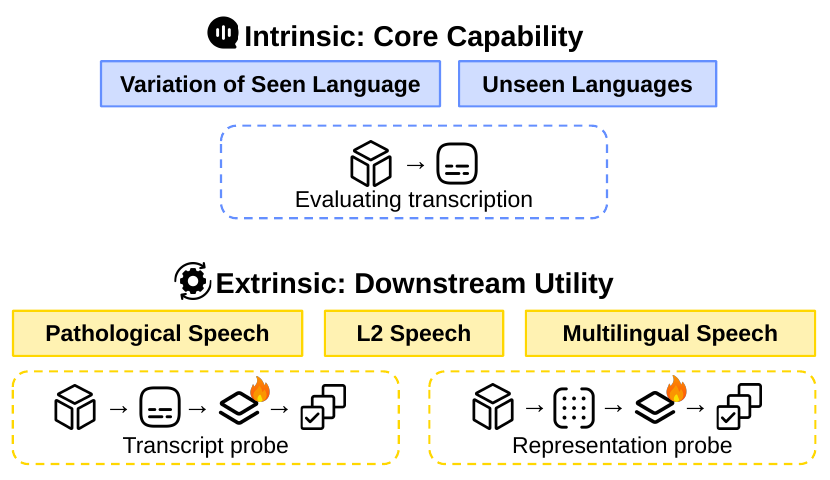
\includegraphics[width=0.82\columnwidth]{figs/prism_overview.png}
  \caption{The PRiSM evaluation framework. We build on the extrinsic part: the transcript probe (left) and the representation probe (right). Reproduced from \citet{bharadwaj2026prism}, Figure~1.}
  \label{fig:prism}
\end{figure}

\begin{figure*}[t]
  \centering
  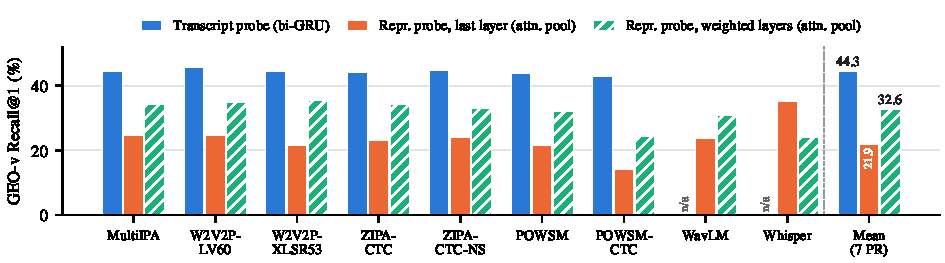
\includegraphics[width=\textwidth]{figs/geov_gap.pdf}
  \caption{\geov{} Recall@1 for each PR model, plotted from Tables~4 and~7 of \citet{bharadwaj2026prism}. Averaged over the seven PR models, a weighted sum over layers lifts the representation probe from 21.9 to 32.6, which closes about half of its gap to the transcript probe (44.3). The remaining gap of about 12 points is what our study tries to explain. WavLM and Whisper produce no phones, so they have no transcript probe.}
  \label{fig:gap}
\end{figure*}

\paragraph{An overlooked clue in the appendix.} Appendix~F of PRiSM repeats the RP with a learned weighted sum over all layers. On \geov, this raises Recall@1 by 8.8 to 14.0 points for every PR model (Figure~\ref{fig:gap}). So part of the TP--RP gap comes from \emph{which layer} is probed, not from order. Any test of the order hypothesis must control for layer choice. We are not aware of prior work that separates these two factors.

%======================================================================
\section{Objectives}
\label{sec:objectives}

Our goal is to find out which phonetic information the two probes use to place a Hindi-belt speaker on the map, with a focus on Haryanvi. We pose three research questions.

\begin{description}[leftmargin=0pt,labelindent=0pt,itemsep=2pt]
  \item[RQ1 (Order).] Is the TP--RP gap caused by phone order? We test this with a $2\times2$ design: \{transcript, representation\} $\times$ \{order-aware, order-free\} probes, with layer choice held fixed.
  \item[RQ2 (Duration).] Do PR models and their probes detect consonant gemination in Haryanvi, e.g., \textipa{[ku:lar]} $\rightarrow$ \textipa{[kullar]} \citep{devi2021haryanvi}? Does detected doubling match a longer acoustic closure?
  \item[RQ3 (Melody).] Does adding pitch and energy contours to the transcript probe improve geolocation, or are segmental cues enough \citep{gumperz1958}?
\end{description}

\noindent The concrete objectives are:
\begin{enumerate}[label=\textbf{O\arabic*.}]
  \item Reproduce the PRiSM \geov{} TP and RP baselines for two PR models, within 2 Recall@1 points of the published numbers.
  \item Run the order ablations of RQ1 and report which factor (order, layer, or discretization) explains the gap.
  \item Measure gemination in Haryana speech, both in model outputs and acoustically, and test whether the probes use it (RQ2).
  \item Measure the added value of prosodic features for dialect geolocation (RQ3).
  \item Release code and a per-state error analysis for the Haryana region and its neighbours.
\end{enumerate}

%======================================================================
\section{Datasets}
\label{sec:data}

Table~\ref{tab:data} lists the data and pretrained models we need. All are public; the two datasets require accepting their terms on Hugging Face. The main dataset is Vaani-Hi, released by the PRiSM authors. It covers 12 Hindi-belt states, including Haryana and its neighbours Delhi, Punjab, Chandigarh, Rajasthan, and Uttar Pradesh. Each location is a pincode with more than 450 utterances; the label is the pincode's mean latitude and longitude. Splits are made within each pincode (75/10/15), and audio is resampled to 16\,kHz and clipped to 20\,s.

\begin{table*}[t]
\centering
\footnotesize
\setlength{\tabcolsep}{2.7pt}
\begin{tabular}{@{}ll>{\ttfamily\scriptsize}lll>{\centering\arraybackslash}p{1.15cm}@{}}
\toprule
\textbf{Resource} & \textbf{Role} & \normalfont\footnotesize\textbf{Hugging Face / GitHub ID} & \textbf{Licence, access} & \textbf{Size} & \textbf{Down\-loaded?} \\
\midrule
Vaani-Hi & \geov{} task & changelinglab/vaani-hi-geo & CC BY 4.0, gated & 6.61\,GB & No$^\dagger$ \\
Vaani (4 districts) & Gemination check & ARTPARK-IISc/Vaani & CC BY 4.0, gated & 92.3\,GB & No \\
W2V2P-LV60 & PR model & facebook/wav2vec2-lv-60-espeak-cv-ft & Apache-2.0 & 317M params & Yes \\
ZIPA-CTC-NS & PR model & anyspeech/zipa-large-crctc-ns-800k & MIT & 300M params & Yes \\
Whisper-small & RP baseline & openai/whisper-small & Apache-2.0 & 244M params & Yes \\
PRiSM code & Probe recipes & github.com/changelinglab/prism & public & -- & Yes \\
Parselmouth & F0, duration & pypi: praat-parselmouth & GPL & -- & Yes \\
\bottomrule
\end{tabular}
\caption{Datasets, models, and tools; availability checked on 9 October 2026. $^\dagger$Access requested; approval pending. Vaani-Hi splits are 19,780 / 2,668 / 3,985 utterances (train / validation / test; Table~5 of \citealp{bharadwaj2026prism}). The full Vaani Phase~1 release is 7.21\,TB of audio, of which we need only the transcribed speech (55.9\,h) of four districts: Rohtak (16.6\,h), Jhajjar (15.1\,h), Charkhi Dadri (13.9\,h), and New Delhi (10.4\,h). Vaani stores audio in one folder per state and district, so we download only these four folders (92.3\,GB). The PRiSM README still lists Vaani-Hi as \texttt{shikhar7ssu/vaani-hi-geo} (``to be released''); the released copy is the one above.}
\label{tab:data}
\end{table*}

Each Vaani-Hi utterance carries its pincode, coordinates, state, district, gender, and spoken-language label, but no speaker ID or transcript. The Phase~1 Vaani release adds transcribed speech from three Haryana districts (Rohtak, Jhajjar, and Charkhi Dadri), which we compare against New Delhi in the gemination analysis of \S\ref{sec:ling}. Unlike Vaani-Hi, these files give speaker IDs for 21--31\% of utterances, so this analysis can hold out whole speakers. The PRiSM toolkit already ships \geov{} probing recipes for all three of our models, loaded from the checkpoints in Table~\ref{tab:data}.

We pick W2V2P-LV60 \citep{xu2022simple} because the PRiSM attribution analysis shows it outputs doubled phones for Haryanvi speech (Figure~\ref{fig:attr}). We pick ZIPA-CTC-NS \citep{zhu2025zipa} because it is the strongest model overall in PRiSM. Whisper-small \citep{radford2023whisper} has the best last-layer RP on \geov{} (35.0) but drops to 24.0 with a weighted layer sum, the only model to do so; we keep it to study this anomaly.

%======================================================================
\section{Linguistic Aspects and Analysis Plan}
\label{sec:ling}

The \geov{} task asks one linguistic question: which properties of speech mark where a Hindi-belt speaker is from? Gumperz showed that Hindi dialects differ in their phonology, not only in vocabulary \citep{gumperz1958}. Dialects can also share a phone inventory but differ in how often phones occur and in which order \citep{shim2024phonotactic}. We study four phonetic levels, from segment to utterance.

\subsection{Phonotactics and phone order (RQ1)}
If order matters, a probe must see \emph{which phone follows which}. Attention pooling computes a weighted average of frames, so it cannot model such sequences. Adding positional encodings \citep{vaswani2017attention} before the pooling does not fix this: the pooled vector then only carries an average position. Order sensitivity needs frames to interact \emph{before} pooling. Table~\ref{tab:probes} lists the probes we compare. We keep the number of trainable parameters similar across probes and run each RP variant on both the last layer and a weighted layer sum.

\begin{table}[t]
\centering
\small
\setlength{\tabcolsep}{4pt}
\begin{tabular}{@{}llc@{}}
\toprule
\textbf{Probe} & \textbf{Input} & \textbf{Sees order?} \\
\midrule
TP-GRU (PRiSM) & phone string & yes \\
TP-Bigram & phone bigram counts & local only \\
TP-Shuffle & permuted phones & no \\
\midrule
RP-Attn (PRiSM) & hidden states & no \\
RP-Attn+PE & hidden states + PE & weak \\
RP-GRU & hidden states & yes \\
RP-Transformer & hidden states + PE & yes \\
RP-ChunkShuffle & permuted 200\,ms chunks & local only \\
\bottomrule
\end{tabular}
\caption{Probe variants for RQ1. Each RP variant is run on the last layer and on a learned weighted sum of the layers selected by a layer sweep (\S\ref{sec:plan}).}
\label{tab:probes}
\end{table}

TP-Shuffle is the cheapest and most decisive test: each TP run takes at most 15 minutes in PRiSM. If TP-Shuffle stays close to TP-GRU, the transcript probe mostly relies on \emph{which phones occur and how often}, and the order hypothesis is weakened. If it drops sharply, and RP-GRU and RP-Transformer beat RP-Attn, the hypothesis is supported.

\subsection{Segment duration: gemination (RQ2)}
Hindi contrasts single and doubled (geminate) consonants, and geminates have significantly longer closures than singletons \citep{ohala2007geminates}. In the Bangru dialect of Haryanvi, speakers double consonants that are single in standard Hindi \citep{devi2021haryanvi}, e.g., \textipa{[r@.k\super{h}a:]} $\rightarrow$ \textipa{[r@k.k\super{h}a:]} (``kept''). PRiSM shows one such utterance where W2V2P-LV60 outputs \textipa{[ll]} and \textipa{[kk]}, and the TP attributes its decision to one of the doubled phones (Figure~\ref{fig:attr}). The authors leave a detailed analysis to future work. We will:
\begin{enumerate}
  \item \textbf{Count doubling in model output.} Compute a doubled-phone rate (DPR) per utterance: the share of consonants written twice or with a length mark. Compare DPR across states and test if Haryana is higher than its neighbours.
  \item \textbf{Check it acoustically.} Sample about 200 doubled and 200 single tokens from Haryana and Delhi speech, verify them by listening, and measure closure duration in Praat \citep{boersma2024praat}. This tells us whether model doubling tracks a real duration difference.
  \item \textbf{Find where it is encoded.} Train a frame-level linear probe for geminate vs.\ single closure at every layer, following layer-wise analysis of speech models \citep{pasad2021layerwise}. \citet{wells2022phonetic} found that the closure and release of a plosive are often represented by different HuBERT units. If gemination is clearest in middle layers, this would also explain why the weighted layer sum helps on \geov.
  \item \textbf{Attribute.} Repeat the integrated-gradients analysis of PRiSM \citep{sundararajan2017axiomatic} over the whole Haryana test set, and report how often top-attributed phones are doubled consonants.
\end{enumerate}

\begin{figure}[t]
  \centering
  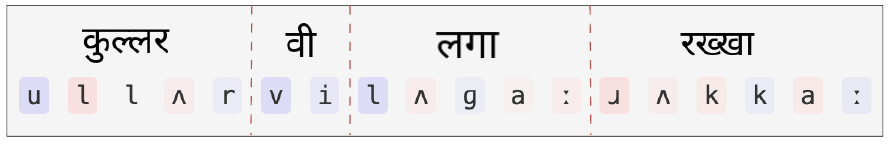
\includegraphics[width=\columnwidth]{figs/prism_attribution.png}
  \caption{Integrated-gradients attribution on a Vaani utterance. Red supports and blue opposes the correct location. W2V2P-LV60 outputs the doubled phones \textipa{[ll]} and \textipa{[kk]}. Reproduced from \citet{bharadwaj2026prism}, Figure~4.}
  \label{fig:attr}
\end{figure}

\subsection{Syllable structure}
Gemination also moves a syllable boundary: \textipa{[r@.k\super{h}a:]} has an open first syllable, and \textipa{[r@k.k\super{h}a:]} has a closed one. We will syllabify the predicted transcripts with a sonority-based rule and compute the share of closed syllables per utterance. This gives a second, syllable-level view of the same dialect feature, and links our study to syllabification, which is part of this course.

\subsection{Intonation (RQ3)}
Listeners use intonation to tell dialects apart \citep{vicenik2013intonation}, and intonation differs across regional varieties \citep{grabe2002intonational}. Transcripts remove this signal. Following the syllable-level prosodic features used for stress detection by \citet{bernhard2022stress}, we extract F0 (in semitones relative to the speaker median), intensity, and voiced-segment durations with Parselmouth \citep{jadoul2018parselmouth}. A small bi-GRU encodes these contours. We compare TP alone, prosody alone, and their late fusion.

\subsection{Evaluation protocol}
We report Recall@1 and mean great-circle error in km, as in PRiSM, plus per-state Recall@1 for Haryana and its neighbours. All numbers are mean $\pm$ standard deviation over 5 seeds. Differences between probes are tested with a paired bootstrap over test utterances (1,000 resamples). To check that a strong probe is not just memorizing, we add a control task with shuffled location labels \citep{hewitt2019control}. Vaani-Hi has no speaker IDs and its splits are random within each pincode, so the same speaker may appear in train and test. We group utterances by voice similarity, using speaker-embedding clusters without identifying anyone, and also report results on this approximately speaker-disjoint split.

%======================================================================
\section{Execution Plan}
\label{sec:plan}

\paragraph{Expected outcomes.} Table~\ref{tab:outcomes} states in advance how we will read each result, so that every outcome is informative.

\begin{table}[t]
\centering
\small
\begin{tabularx}{\columnwidth}{@{}>{\raggedright\arraybackslash}p{0.44\columnwidth}X@{}}
\toprule
\textbf{If we observe} & \textbf{We conclude} \\
\midrule
TP-Shuffle $\approx$ TP-GRU & Order is not needed; TP uses phone frequencies. \\
TP-Shuffle $\ll$ TP-GRU, and RP-GRU $\gg$ RP-Attn & Order explains the gap (PRiSM hypothesis holds). \\
RP-Attn+PE $\approx$ RP-Attn & Positional encoding alone is not enough. \\
Order-aware RP still $<$ TP & Discretization helps by removing speaker and channel variation. \\
DPR higher in Haryana, and tracks closure duration & Models capture a real dialect feature. \\
Geminates peak in middle layers & Explains the weighted-sum gain. \\
TP+Prosody $>$ TP (significant) & Intonation adds dialect information. \\
\bottomrule
\end{tabularx}
\caption{Pre-registered readings of possible results.}
\label{tab:outcomes}
\end{table}

\paragraph{Timeline.} Table~\ref{tab:timeline} maps the work to the calendar.

\begin{table}[t]
\centering
\small
\begin{tabularx}{\columnwidth}{@{}lX@{}}
\toprule
\textbf{Dates} & \textbf{Work} \\
\midrule
10--16 Oct & Download the four Vaani district folders; extract last-layer features. \\
17--26 Oct & Reproduce TP and RP baselines (O1). \\
27 Oct--2 Nov & TP-Shuffle and TP-Bigram; DPR per state. \\
\textbf{3 Nov} & \textbf{Mid evaluation}: baselines, first RQ1 result, DPR map. \\
4--17 Nov & Order-aware RP probes with layer control (O2); Praat measurements and layer-wise geminate probe (O3). \\
18--30 Nov & Prosody stream and fusion (O4); attribution; syllable analysis. \\
\textbf{4 Dec} & \textbf{End evaluation}: report, code, error analysis (O5). \\
\bottomrule
\end{tabularx}
\caption{Project timeline.}
\label{tab:timeline}
\end{table}

\paragraph{Division of work.} \emph{Mohit Kumar Singh} leads the modelling side: feature extraction, probe variants, and RQ1. \emph{Nidhi Vaidya} leads the phonetic side: DPR, Praat measurements, syllabification, and prosodic features (RQ2, RQ3). Both members reproduce the baselines together, and each checks the other's results.

\paragraph{Compute.} We freeze all PR models and train only small probes. PRiSM reports at most 15 minutes per TP run and 3 hours per RP run on one 40\,GB GPU. Storage, not GPU time, is the main cost: one layer of W2V2P-LV60 (24 layers, 1024 dimensions) over Vaani-Hi takes 10--20\,GB in half precision, and all 25 layers would take hundreds of GB. So we first average each layer over time into one vector per utterance and run a cheap layer sweep, then cache full frame sequences only for the last layer and the two or three most informative layers. Weighted-layer probes use this selected set. Transcription, TP runs, and the phonetic analyses fit on a single consumer GPU; the RP sweep (about 150 runs) runs on the institute GPU cluster.

\paragraph{Risks.} (i) Both PR vocabularies can mark consonant length (e.g., \textipa{[k:]}), but a model may still rarely use it on this speech; RQ2 then relies on W2V2P-LV60 and the acoustic measurements. (ii) If Vaani-Hi access is delayed, we rebuild an approximate copy with the PRiSM sampling script. (iii) If compute is short, we drop RP-Transformer and keep RP-GRU as the order-aware RP.

\section*{Limitations}
Vaani-Hi labels a recording by location and language, not by dialect, so a speaker living in Haryana may not speak Haryanvi (only 4--9\% of our Haryana utterances are labelled Haryanvi). Speaker overlap between splits can only be estimated, not removed exactly. Our gemination analysis covers one documented feature of one dialect group. The manual check of 400 tokens is small, and we will report agreement between the two members on a shared subset.

\section*{Ethics Statement}
Locating a speaker from their voice can be misused, e.g., for profiling. We use only public data under its licence, report results at the state and pincode level, and do not attempt to identify individuals. We follow the ethics statement of the base paper.

\bibliography{custom}

\end{document}
